% Generated by Sphinx.
\def\sphinxdocclass{report}
\documentclass[letterpaper,10pt,english]{sphinxmanual}
\usepackage[utf8]{inputenc}
\DeclareUnicodeCharacter{00A0}{\nobreakspace}
\usepackage[T1]{fontenc}
\usepackage{babel}
\usepackage{times}
\usepackage[Bjarne]{fncychap}
\usepackage{longtable}
\usepackage{sphinx}
\usepackage{multirow}


\title{imalse Documentation}
\date{August 19, 2012}
\release{0.0 alpha}
\author{Jing Conan Wang}
\newcommand{\sphinxlogo}{}
\renewcommand{\releasename}{Release}
\makeindex

\makeatletter
\def\PYG@reset{\let\PYG@it=\relax \let\PYG@bf=\relax%
    \let\PYG@ul=\relax \let\PYG@tc=\relax%
    \let\PYG@bc=\relax \let\PYG@ff=\relax}
\def\PYG@tok#1{\csname PYG@tok@#1\endcsname}
\def\PYG@toks#1+{\ifx\relax#1\empty\else%
    \PYG@tok{#1}\expandafter\PYG@toks\fi}
\def\PYG@do#1{\PYG@bc{\PYG@tc{\PYG@ul{%
    \PYG@it{\PYG@bf{\PYG@ff{#1}}}}}}}
\def\PYG#1#2{\PYG@reset\PYG@toks#1+\relax+\PYG@do{#2}}

\expandafter\def\csname PYG@tok@gd\endcsname{\def\PYG@tc##1{\textcolor[rgb]{0.63,0.00,0.00}{##1}}}
\expandafter\def\csname PYG@tok@gu\endcsname{\let\PYG@bf=\textbf\def\PYG@tc##1{\textcolor[rgb]{0.50,0.00,0.50}{##1}}}
\expandafter\def\csname PYG@tok@gt\endcsname{\def\PYG@tc##1{\textcolor[rgb]{0.00,0.25,0.82}{##1}}}
\expandafter\def\csname PYG@tok@gs\endcsname{\let\PYG@bf=\textbf}
\expandafter\def\csname PYG@tok@gr\endcsname{\def\PYG@tc##1{\textcolor[rgb]{1.00,0.00,0.00}{##1}}}
\expandafter\def\csname PYG@tok@cm\endcsname{\let\PYG@it=\textit\def\PYG@tc##1{\textcolor[rgb]{0.25,0.50,0.56}{##1}}}
\expandafter\def\csname PYG@tok@vg\endcsname{\def\PYG@tc##1{\textcolor[rgb]{0.73,0.38,0.84}{##1}}}
\expandafter\def\csname PYG@tok@m\endcsname{\def\PYG@tc##1{\textcolor[rgb]{0.13,0.50,0.31}{##1}}}
\expandafter\def\csname PYG@tok@mh\endcsname{\def\PYG@tc##1{\textcolor[rgb]{0.13,0.50,0.31}{##1}}}
\expandafter\def\csname PYG@tok@cs\endcsname{\def\PYG@tc##1{\textcolor[rgb]{0.25,0.50,0.56}{##1}}\def\PYG@bc##1{\setlength{\fboxsep}{0pt}\colorbox[rgb]{1.00,0.94,0.94}{\strut ##1}}}
\expandafter\def\csname PYG@tok@ge\endcsname{\let\PYG@it=\textit}
\expandafter\def\csname PYG@tok@vc\endcsname{\def\PYG@tc##1{\textcolor[rgb]{0.73,0.38,0.84}{##1}}}
\expandafter\def\csname PYG@tok@il\endcsname{\def\PYG@tc##1{\textcolor[rgb]{0.13,0.50,0.31}{##1}}}
\expandafter\def\csname PYG@tok@go\endcsname{\def\PYG@tc##1{\textcolor[rgb]{0.19,0.19,0.19}{##1}}}
\expandafter\def\csname PYG@tok@cp\endcsname{\def\PYG@tc##1{\textcolor[rgb]{0.00,0.44,0.13}{##1}}}
\expandafter\def\csname PYG@tok@gi\endcsname{\def\PYG@tc##1{\textcolor[rgb]{0.00,0.63,0.00}{##1}}}
\expandafter\def\csname PYG@tok@gh\endcsname{\let\PYG@bf=\textbf\def\PYG@tc##1{\textcolor[rgb]{0.00,0.00,0.50}{##1}}}
\expandafter\def\csname PYG@tok@ni\endcsname{\let\PYG@bf=\textbf\def\PYG@tc##1{\textcolor[rgb]{0.84,0.33,0.22}{##1}}}
\expandafter\def\csname PYG@tok@nl\endcsname{\let\PYG@bf=\textbf\def\PYG@tc##1{\textcolor[rgb]{0.00,0.13,0.44}{##1}}}
\expandafter\def\csname PYG@tok@nn\endcsname{\let\PYG@bf=\textbf\def\PYG@tc##1{\textcolor[rgb]{0.05,0.52,0.71}{##1}}}
\expandafter\def\csname PYG@tok@no\endcsname{\def\PYG@tc##1{\textcolor[rgb]{0.38,0.68,0.84}{##1}}}
\expandafter\def\csname PYG@tok@na\endcsname{\def\PYG@tc##1{\textcolor[rgb]{0.25,0.44,0.63}{##1}}}
\expandafter\def\csname PYG@tok@nb\endcsname{\def\PYG@tc##1{\textcolor[rgb]{0.00,0.44,0.13}{##1}}}
\expandafter\def\csname PYG@tok@nc\endcsname{\let\PYG@bf=\textbf\def\PYG@tc##1{\textcolor[rgb]{0.05,0.52,0.71}{##1}}}
\expandafter\def\csname PYG@tok@nd\endcsname{\let\PYG@bf=\textbf\def\PYG@tc##1{\textcolor[rgb]{0.33,0.33,0.33}{##1}}}
\expandafter\def\csname PYG@tok@ne\endcsname{\def\PYG@tc##1{\textcolor[rgb]{0.00,0.44,0.13}{##1}}}
\expandafter\def\csname PYG@tok@nf\endcsname{\def\PYG@tc##1{\textcolor[rgb]{0.02,0.16,0.49}{##1}}}
\expandafter\def\csname PYG@tok@si\endcsname{\let\PYG@it=\textit\def\PYG@tc##1{\textcolor[rgb]{0.44,0.63,0.82}{##1}}}
\expandafter\def\csname PYG@tok@s2\endcsname{\def\PYG@tc##1{\textcolor[rgb]{0.25,0.44,0.63}{##1}}}
\expandafter\def\csname PYG@tok@vi\endcsname{\def\PYG@tc##1{\textcolor[rgb]{0.73,0.38,0.84}{##1}}}
\expandafter\def\csname PYG@tok@nt\endcsname{\let\PYG@bf=\textbf\def\PYG@tc##1{\textcolor[rgb]{0.02,0.16,0.45}{##1}}}
\expandafter\def\csname PYG@tok@nv\endcsname{\def\PYG@tc##1{\textcolor[rgb]{0.73,0.38,0.84}{##1}}}
\expandafter\def\csname PYG@tok@s1\endcsname{\def\PYG@tc##1{\textcolor[rgb]{0.25,0.44,0.63}{##1}}}
\expandafter\def\csname PYG@tok@gp\endcsname{\let\PYG@bf=\textbf\def\PYG@tc##1{\textcolor[rgb]{0.78,0.36,0.04}{##1}}}
\expandafter\def\csname PYG@tok@sh\endcsname{\def\PYG@tc##1{\textcolor[rgb]{0.25,0.44,0.63}{##1}}}
\expandafter\def\csname PYG@tok@ow\endcsname{\let\PYG@bf=\textbf\def\PYG@tc##1{\textcolor[rgb]{0.00,0.44,0.13}{##1}}}
\expandafter\def\csname PYG@tok@sx\endcsname{\def\PYG@tc##1{\textcolor[rgb]{0.78,0.36,0.04}{##1}}}
\expandafter\def\csname PYG@tok@bp\endcsname{\def\PYG@tc##1{\textcolor[rgb]{0.00,0.44,0.13}{##1}}}
\expandafter\def\csname PYG@tok@c1\endcsname{\let\PYG@it=\textit\def\PYG@tc##1{\textcolor[rgb]{0.25,0.50,0.56}{##1}}}
\expandafter\def\csname PYG@tok@kc\endcsname{\let\PYG@bf=\textbf\def\PYG@tc##1{\textcolor[rgb]{0.00,0.44,0.13}{##1}}}
\expandafter\def\csname PYG@tok@c\endcsname{\let\PYG@it=\textit\def\PYG@tc##1{\textcolor[rgb]{0.25,0.50,0.56}{##1}}}
\expandafter\def\csname PYG@tok@mf\endcsname{\def\PYG@tc##1{\textcolor[rgb]{0.13,0.50,0.31}{##1}}}
\expandafter\def\csname PYG@tok@err\endcsname{\def\PYG@bc##1{\setlength{\fboxsep}{0pt}\fcolorbox[rgb]{1.00,0.00,0.00}{1,1,1}{\strut ##1}}}
\expandafter\def\csname PYG@tok@kd\endcsname{\let\PYG@bf=\textbf\def\PYG@tc##1{\textcolor[rgb]{0.00,0.44,0.13}{##1}}}
\expandafter\def\csname PYG@tok@ss\endcsname{\def\PYG@tc##1{\textcolor[rgb]{0.32,0.47,0.09}{##1}}}
\expandafter\def\csname PYG@tok@sr\endcsname{\def\PYG@tc##1{\textcolor[rgb]{0.14,0.33,0.53}{##1}}}
\expandafter\def\csname PYG@tok@mo\endcsname{\def\PYG@tc##1{\textcolor[rgb]{0.13,0.50,0.31}{##1}}}
\expandafter\def\csname PYG@tok@mi\endcsname{\def\PYG@tc##1{\textcolor[rgb]{0.13,0.50,0.31}{##1}}}
\expandafter\def\csname PYG@tok@kn\endcsname{\let\PYG@bf=\textbf\def\PYG@tc##1{\textcolor[rgb]{0.00,0.44,0.13}{##1}}}
\expandafter\def\csname PYG@tok@o\endcsname{\def\PYG@tc##1{\textcolor[rgb]{0.40,0.40,0.40}{##1}}}
\expandafter\def\csname PYG@tok@kr\endcsname{\let\PYG@bf=\textbf\def\PYG@tc##1{\textcolor[rgb]{0.00,0.44,0.13}{##1}}}
\expandafter\def\csname PYG@tok@s\endcsname{\def\PYG@tc##1{\textcolor[rgb]{0.25,0.44,0.63}{##1}}}
\expandafter\def\csname PYG@tok@kp\endcsname{\def\PYG@tc##1{\textcolor[rgb]{0.00,0.44,0.13}{##1}}}
\expandafter\def\csname PYG@tok@w\endcsname{\def\PYG@tc##1{\textcolor[rgb]{0.73,0.73,0.73}{##1}}}
\expandafter\def\csname PYG@tok@kt\endcsname{\def\PYG@tc##1{\textcolor[rgb]{0.56,0.13,0.00}{##1}}}
\expandafter\def\csname PYG@tok@sc\endcsname{\def\PYG@tc##1{\textcolor[rgb]{0.25,0.44,0.63}{##1}}}
\expandafter\def\csname PYG@tok@sb\endcsname{\def\PYG@tc##1{\textcolor[rgb]{0.25,0.44,0.63}{##1}}}
\expandafter\def\csname PYG@tok@k\endcsname{\let\PYG@bf=\textbf\def\PYG@tc##1{\textcolor[rgb]{0.00,0.44,0.13}{##1}}}
\expandafter\def\csname PYG@tok@se\endcsname{\let\PYG@bf=\textbf\def\PYG@tc##1{\textcolor[rgb]{0.25,0.44,0.63}{##1}}}
\expandafter\def\csname PYG@tok@sd\endcsname{\let\PYG@it=\textit\def\PYG@tc##1{\textcolor[rgb]{0.25,0.44,0.63}{##1}}}

\def\PYGZbs{\char`\\}
\def\PYGZus{\char`\_}
\def\PYGZob{\char`\{}
\def\PYGZcb{\char`\}}
\def\PYGZca{\char`\^}
\def\PYGZam{\char`\&}
\def\PYGZlt{\char`\<}
\def\PYGZgt{\char`\>}
\def\PYGZsh{\char`\#}
\def\PYGZpc{\char`\%}
\def\PYGZdl{\char`\$}
\def\PYGZti{\char`\~}
% for compatibility with earlier versions
\def\PYGZat{@}
\def\PYGZlb{[}
\def\PYGZrb{]}
\makeatother

\begin{document}

\maketitle
\tableofcontents
\phantomsection\label{index::doc}



\chapter{Introduction}
\label{index:introduction}\label{index:welcome-to-imalse-s-documentation}
IMALSE (\textbf{I}ntegrated   \textbf{MAL}ware \textbf{S}imulator and \textbf{E}mulator) is
a framework to help researchers to implement prototype of botnet based network
malware. Researchers just need to implement the malware behaviour once and then
it can run the following three modes:
\begin{itemize}
\item {} 
\textbf{emulation mode}: In this mode, each copy of imalse will behave exactly
like a real malware. You can install it in a real machine, or in a virtual
machine and set up a testbed to test the characteristic of the
malware.(Don't use it to attack other people's machines;) ) {[}\textbf{Note}: you
can potentially work with Common Open Research Emulator to emulate a lot
of nodes in one machine{]}

\item {} 
\textbf{netns3 simulation mode}:  You can specifiy the topology of the network
and the ip addresses of each node in this mode. IMALSE will launch virtual
machines (linux namespace) for each node in the network and construct  the
network automatically. All virtualized nodes will connect to \textbf{NS3}
through tapbridge and all traffic will consume there. The simulation will
be in real time. It is based on \href{http://www.nsnam.org/wiki/index.php/HOWTO\_use\_Linux\_namespaces\_with\_ns-3}{netns3}
project.

\item {} 
\textbf{pure ns3 simulation mode}: No virtual machince will be launched for the
pure ns3 simulation mode, the whole simulation will be done in \href{http://www.nsnam.org/}{ns3}. ns3 default scheduler will be used instead of
the real time scheduler in netns3 case, which saves much time. One
simulation day may only consume several real seconds.

\end{itemize}

{\hfill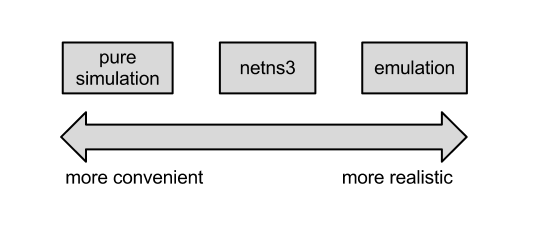
\includegraphics{imalse-abstract.png}\hfill}


\section{Typical Use Case}
\label{index:typical-use-case}
Suppose Conan is a Ph.D student who has proposed a novel anomaly detection
technique for Internet traffic. He wants to demostrate the usefulness of this
approach. To do this, he designs a scenario that 100 client computers accessing
a server through the internet, 10 of which had already been compromised and
controlled by botmaster through botnet. At some point, the botmaster will
initiate a ddos attack by asking all compromised computers to send ping requests
to the servers. The anomaly detection technique requires all the incoming and
outcoming traffic of the server for at least two days.

How can he collect the data he want? imalse provides different solutions at
different abstract level. He decides to use \textbf{TopoSimExperiment} in which he
can load some topology file generated by \href{http://topology.eecs.umich.edu/inet/}{Inet} topology generator and select
\textbf{ddos\_ping\_attack} attacking scenario from the imalse software which provide
exactly what he wants.

The first question is since the method is not mature, Conan wants to test it
under different parameter combinations. It will be forever if each simulation
takes more than two days. Fortunately, by running the simulation under \textbf{pure
ns3 simulation mode} Conan can finish one simulation with less 100 real
seconds, though the time has past for more than two days in the simulator.

After extensive testing, Conan has been quite confident about the performance of
the anomaly detection techinique now. But he is still a little bit worried about
whether the result of ns3 is convincing enough. As a result, he run a complete
simulation under \textbf{netns3 simulation model} and collect data. Of course, this
time it runs more than two days, but he doesn't care that much because he only
need to run it for very few times. Conan generates some plots and writes a
paper with data of \textbf{netns3 simulation model} and satisfied with this.

A rich company named NetSecurity reads this paper and think it is a good method.
They want to deploy it but need more realistic test before deployment, so they
decide to test it under their intranet. They ask Conan for a copy of the code
and select several computer in the intranet to join the botnet, each computer
run an independent copy of imalse under \textbf{emulation client mode}, there is a
computer serving as botmster and running a imalse under \textbf{emulation server
model}(the server refers to the C\&C server in the botnet). The data of
attacked server is recorded and analyzed with Conan's tools. It turns out to be
good, and the Company decide to use this method.

As a lazy Ph.D student, Conan just need to write one copy of code to describe
the secnario during the whole process. With the help of imalse, he can have more
time to sleep and enjoy the classical music. :)


\chapter{Description:}
\label{index:description}
To support the variety of modes noted above, Imalse design in a way that to
seperate the botnet mechanism and the network.

The general structure of Imalse is shown in the following figure:

{\hfill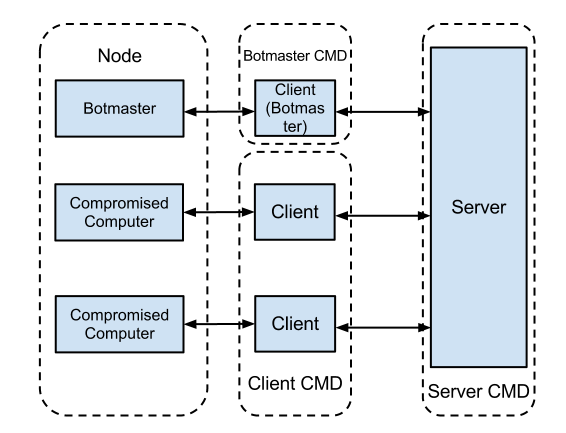
\includegraphics{genearal-structure.png}\hfill}

\textbf{Node} and \textbf{C}ommand \textbf{M}eta \textbf{D}escription are the two key concepts
in the design.  \textbf{Node} is the abstraction of a real computer. A node should
support:
\begin{itemize}
\item {} 
\textbf{Basic Utility Functions}: serveral basic utility calls, including
getting the system time, make node sleep, so on so forth

\item {} 
\textbf{Socket API} this is require to implement basic

\item {} 
\textbf{File System}

\item {} 
\textbf{Higher Level Application}

\end{itemize}

There is a abstract base class in core module named \textbf{BaseNode} that define the
all APIs a node need to overload. If you want to extend the framework to support
other type of simulator, please subclass \textbf{BaseNode} and implement all the
virtual functions.

a command is a basic event. \textbf{C}ommand \textbf{M}eta \textbf{D}escription defines a
set of commands for a node, namely it defines what event a node can generate.
There are three types of \textbf{CMD}s:
\begin{enumerate}
\item {} 
Server \textbf{CMD}: Command meta description for the server. Server usually
will waiting attack command from botmaster and send corresponding commands to
clients.

\item {} 
Client \textbf{CMD}: Client will wait command from server and do
correspondingactions in user's comoputer. What a Client can do depends on
the Node \textbf{API}

\item {} 
Botmaster \textbf{CMD}: Botmaster is actually a special client with higher
privilege. Botmaster should verify itself by sending verify command and
send attack commands to server.

\end{enumerate}

The basic procedure is that the botmaster send commands to the server, the server
translates the commands and send commands to Clients.


\section{Basic Botnet Mechanism:}
\label{index:basic-botnet-mechanism}
In \textbf{core} module, imalse provides a basic framework for the botnet and the
support to real network, netns3 and NS3. User can create their own flavor of
botnet by subclassing \textbf{ServerCMD}, \textbf{ClientCMD} and \textbf{BotmasterCMD}, each
flavor is called a new \textbf{scenario}.

The basic botnet mechanism can be described as \textbf{F}inite \textbf{S}tate \textbf{M}achine. The \textbf{FSM} for the \textbf{ClientCMD} is as follows:

{\hfill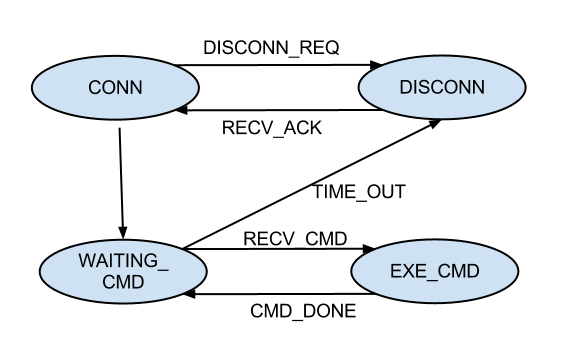
\includegraphics{client_fsm.png}\hfill}


\section{Scenario:}
\label{index:scenario}
As a noted above, user can create their own flavor of \textbf{Botnet}, which is so
called \textbf{scenario}. Currently, Imalse provides two sample \textbf{scenarios}:
\begin{enumerate}
\item {} \begin{description}
\item[{\textbf{ddos\_ping\_flooding}: in this scenario, botmaster can issue \textbf{send\_pings}}] \leavevmode
command to initiate a ddos ping flooding attack to a specific server.

\end{description}

\item {} \begin{description}
\item[{\textbf{file\_exfiltration}: in this scenario, botmaster can request bots to search}] \leavevmode
in the file system with any file that contains a certain pattern,
like \textbf{password}. Whenver an interesting is found, the bot will
upload the file to a ftp server.

\end{description}

\end{enumerate}

To implement a new scenario, you need to create a new folder in scenario
folder. This folder actually is a new module in python. This module should
provide the following classes: \textbf{BotMaster}, \textbf{ClientCMD}, \textbf{ServerCMD}.

You can subclass the BotMaster ClientCMD and ServerCMD in core, which provide a
botnet communication scheme and make the difference of real node, netns3 node
and ns3 sim node to be transparent.
\begin{description}
\item[{An recommendation of implementation}] \leavevmode\begin{enumerate}
\item {} 
put temporal pattern of attack into Botmaster \textbf{CMD}. In other words, in
botmaster \textbf{CMD}, you can specify which attack should happen at what
time. Botmaster can issue a \textbf{file\_scan} attack command every 24 hours,
or according to a possion distribution, etc.

\item {} 
put geographical pattern of attack into Server \textbf{CMD}. In other words,
which clients should join this attack.

\item {} 
put action pattern of attack into Client \textbf{CMD}. A Client command will
define a sequence of node actions, which is unique to this attack.

\end{enumerate}

\end{description}

{\hfill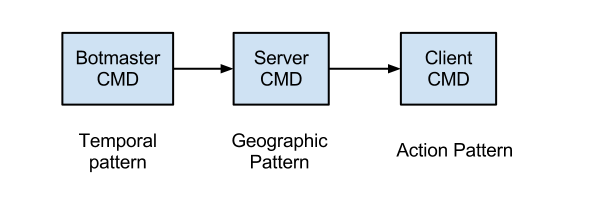
\includegraphics{ImalseCMD.png}\hfill}


\section{Experiment}
\label{index:experiment}
Experiment is only used in \textbf{simulation mode}. Experiments need to do Topology
and network configuration, user behaviour specification. This is usually the
only part user need to code if he is using an existing scenario.

In ROOT/experiments folder, we provide three samples of experiment.
\begin{itemize}
\item {} 
\textbf{StaticRouteExperiment} is a experiment in which a small diamond shape
topology in demoed and the routing tables for all nodes are manually
specificed.

\item {} 
\textbf{TopoExperiment} is a experiment in which you can load topology
generated by some topology generators, like \href{http://topology.eecs.umich.edu/inet/}{Inet} , the ip address of each node
will be automatically assigned. The parameters you can customize are: 1.
\emph{NETWORK\_BASE}, 2. \emph{SERVER\_ADDR}, 3. \emph{IP\_MASK}, 4. \emph{server\_id\_set}, 5.
\emph{botmaster\_id\_set}, 6. \emph{client\_id\_set}, 7. \emph{Delay}, 8. \emph{DataRate}. The
delay and data rate for all links are the same. All parameters are the
static member of \textbf{TopoExperiment} class and you just need to change them
in the code accordingly.  You will need this if you only care about
topology and too lazy to configure the network.

\item {} 
\textbf{ManualTopoExperiment} is simular to \textbf{TopoExperiment}, however, in
\textbf{ManualTopoExperiment}, you can specify the delay and data rate of each
link and also the ip address of every interface. Instead of hard code all
parameters in the code, it will load a configuration script with python
syntax. We provide a GUI editor to create such configuration script.

\end{itemize}

When you want to implement you own version of experiment, you can put it in
ROOT/experiments folder, there is class factory function in the
ROOT/experiments/API.py, when you input the different \textbf{--mode} parameter in the command
line, the class factory function will generate a new experiment class with all
the methods and members you definde with corresponding base class.

Some things you need to pay attention are:
\begin{enumerate}
\item {} \begin{description}
\item[{There is only one experiment for each file. The name of experiment file should}] \leavevmode
have the same name with the experiment class.

\end{description}

\item {} 
The experiment class should declare \textbf{BaseClass}  as the base class

\end{enumerate}

For example, we define the \textbf{TopoExperiment} in \emph{ROOT/experiments/TopoExperiment.py},
the definition of topology experiment is as follows:

\begin{Verbatim}[commandchars=\\\{\}]
\PYG{k}{class} \PYG{n+nc}{TopoExperiment}\PYG{p}{(}\PYG{n}{BaseClass}\PYG{p}{)}\PYG{p}{:}
\end{Verbatim}

It declares BaseClass as the base class, though \textbf{BaseClass} is not defined or
imported in this file. It probably won't pass the syntax checker like \emph{pyflake}
and \emph{pylint}. Actually \textbf{BaseClass} is a placeholder that will later be
replaced by real implementation. To clarify this `strange' code , I will introduce the
implementation details a little bit.  If you don't want to know the reason,
just ignore this part.

\begin{Verbatim}[commandchars=\\\{\}]
\PYG{k}{def} \PYG{n+nf}{experiment\PYGZus{}factory}\PYG{p}{(}\PYG{n}{experiment}\PYG{p}{,} \PYG{n}{mode}\PYG{p}{)}\PYG{p}{:}
    \PYG{n}{BaseClass} \PYG{o}{=} \PYG{n}{mode\PYGZus{}map}\PYG{p}{[}\PYG{n}{mode}\PYG{p}{]}
    \PYG{n}{exper\PYGZus{}fname} \PYG{o}{=} \PYG{n}{settings}\PYG{o}{.}\PYG{n}{ROOT} \PYG{o}{+} \PYG{l+s}{'}\PYG{l+s}{/experiments/}\PYG{l+s}{'} \PYG{o}{+} \PYG{n}{experiment} \PYG{o}{+} \PYG{l+s}{'}\PYG{l+s}{.py}\PYG{l+s}{'}
    \PYG{n+nb}{execfile}\PYG{p}{(}\PYG{n}{exper\PYGZus{}fname}\PYG{p}{,} \PYG{n+nb}{locals}\PYG{p}{(}\PYG{p}{)}\PYG{p}{)}
    \PYG{k}{return} \PYG{n+nb}{locals}\PYG{p}{(}\PYG{p}{)}\PYG{p}{[}\PYG{n}{experiment}\PYG{p}{]}
\end{Verbatim}

The code above is the code of experiment\_factory.  It will dynamically select
the base class according to following map:

\begin{Verbatim}[commandchars=\\\{\}]
\PYG{n}{mode\PYGZus{}map} \PYG{o}{=} \PYG{p}{\PYGZob{}}
        \PYG{l+s}{'}\PYG{l+s}{netns3}\PYG{l+s}{'}\PYG{p}{:}\PYG{n}{ImalseNetnsExperiment}\PYG{p}{,}
        \PYG{l+s}{'}\PYG{l+s}{sim}\PYG{l+s}{'}\PYG{p}{:}\PYG{n}{ImalsePureSimExperiment}\PYG{p}{,}
        \PYG{p}{\PYGZcb{}}
\end{Verbatim}

and then execuate the experiment file according to the name of the experiment it
will load, which is the reason why the name of the file and the experiment class
must be consistant.


\chapter{GUI Support}
\label{index:gui-support}
One important principle of Imalse is ``not reinventing the wheels''. So instead of
implementing a GUI by myself, I take advantage of existing GUI tools,
particually NS3 \href{http://www.nsnam.org/wiki/index.php/PyViz}{PyViz} and
\href{http://cs.itd.nrl.navy.mil/work/core/}{CORE network topology Editor}
( which is again based on
IMUNES network topology editor)
\begin{description}
\item[{The GUI support of Imalse are two folds:}] \leavevmode\begin{enumerate}
\item {} 
It provides a simple visualizer that can visualize the topology and
traffic dynamically. This is based on PyViz.

\item {} 
It provides a complete Network Topology Editor in which you can ``draw'' the
network topology, config the network and export the configuration scripts
for command line to use. This part is based on CORE Network Topology
Editor

\end{enumerate}

\end{description}


\section{Simple Visualizer}
\label{index:simple-visualizer}
The first function is suitable for those who are accustomed to work under command
lines but just need a very simple visualization to check everythings goes right.
You have total control using this, you can implement new command line
settings, and editing network topology and ip address.

Currenly only NS3 pure simulation can be visualized using PyViz. To visualize
the simulation, you just need run the simulation in \emph{sim} mode and add the
\emph{--SimulatorImpl=Visual} in the command. The screenshot of simple visualizer is
as follows:

{\hfill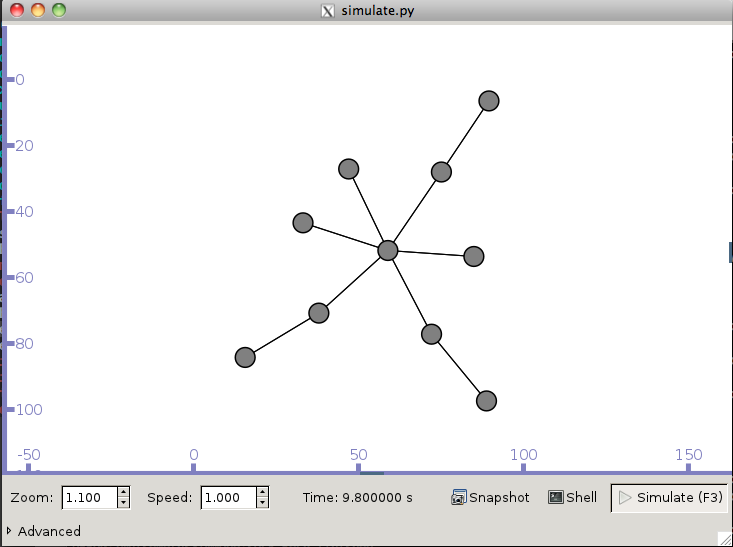
\includegraphics{Visualizer_screenshot.png}\hfill}


\section{Network Topology Editor}
\label{index:network-topology-editor}
One of the most cubersome part of configuration is to 1. create a suitable network
topology. 2. Configure the ip address. 3 and specify the role of each node. You
can definitely do this using commandl line and actually I have tried my best to
make the process easier. For example, in TopologyExperiment, the IP address of
each subnetwork can be automatically assigned. The inet topology generator tool has been
integrated to generate reasonable topology.

However, in many cases, you would prefer to configure by youself instead of
using automated tools. In this case, you will have a lot of tedious typing work
if you use command line tools.

To make the proces easier, the Imalse provide a GUI of topology editor. This GUI
editor is revised from GUI editor of \href{http://cs.itd.nrl.navy.mil/work/core/}{CORE} . A screenshot
is as follows:

{\hfill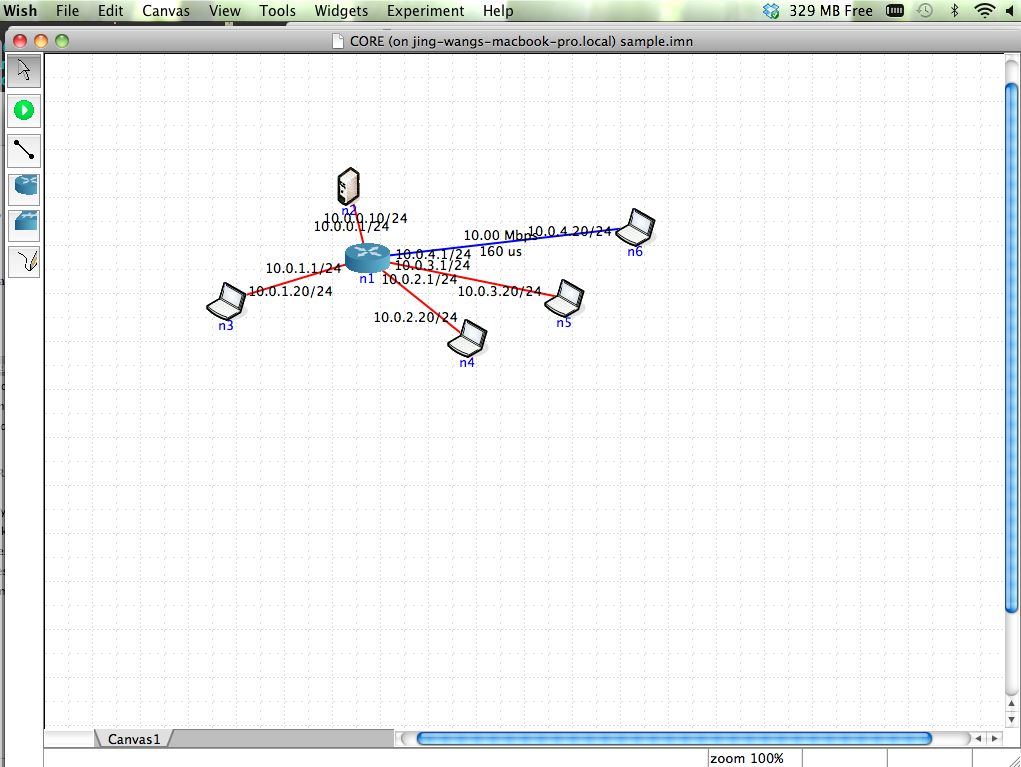
\includegraphics{ImalseGUI.png}\hfill}

please refer to the \href{http://pf.itd.nrl.navy.mil/core/core-html/Using-the-CORE-GUI.html\#Using-the-CORE-GUI}{CORE GUI Manual Page}
and \href{http://imunes.tel.fer.hr/imunes/dl/imunes\_ug\_20110907.pdf}{IMUNES Manual}
for basic usuage of the editor. You can look at the \href{http://www.youtube.com/watch?v=PSXyEXFRSYs\&feature=plcp}{GUI Demo} for the difference.


\chapter{Demo:}
\label{index:demo}
Here are some demo videos
\begin{itemize}
\item {} 
\href{http://www.youtube.com/watch?v=CZ91McFlIvo\&feature=plcp}{Command Line Usage}

\item {} 
\href{http://www.youtube.com/watch?v=PSXyEXFRSYs\&feature=plcp}{GUI usage}

\end{itemize}


\chapter{Source Code:}
\label{index:source-code}
the project is currently hosted on www.bitbucket.org.
To get a copy of the code, please install mercurial first and type

\begin{Verbatim}[commandchars=\\\{\}]
\PYG{n}{hg} \PYG{n}{clone} \PYG{n}{https}\PYG{p}{:}\PYG{o}{/}\PYG{o}{/}\PYG{n}{hbhzwj}\PYG{n+nd}{@bitbucket.org}\PYG{o}{/}\PYG{n}{hbhzwj}\PYG{o}{/}\PYG{n}{imalse}
\end{Verbatim}

in the command line.


\chapter{Installation:}
\label{index:installation}

\section{Installation of NS3}
\label{index:installation-of-ns3}
We recommend you to install a revised version NS3 based on NS3.14.1. We add the
imalse module to this to deal with the packet manipulation. Run the following
command in the bash.

\begin{Verbatim}[commandchars=\\\{\}]
wget https://bitbucket.org/hbhzwj/imalse/downloads/ns-allinone-3.14.1-with-imalse.tar.gz
tar -xzvf ns-allinone-3.14.1-with-imalse.tar.gz
\PYG{n+nb}{cd }ns-allinone-3.14.1-with-imalse
./build.py
\end{Verbatim}

It will check the dependencies first. be careful about the message of and
install the corresponding dependencies. Under Ubuntu 12.04, you can install the dependencies by typing

\begin{Verbatim}[commandchars=\\\{\}]
sudo apt-get install g++ python-dev gccxml python-pygccxml python-pygraphviz python-pygoocanvas
\end{Verbatim}

After building the ns-allinone successfully. There is one more thing you need to
do. The ns3.14.1 has a bug in python binding of dsr, the most recently added
module. You need disable the import of dsr binding in ns3.py.

\begin{Verbatim}[commandchars=\\\{\}]
\PYG{n+nb}{cd }ns-allinone-3.14.1-with-imalse/ns-3.14.1/build/bindings/python/
vi ns3.py
\end{Verbatim}

then comment the

\begin{Verbatim}[commandchars=\\\{\}]
\PYG{k+kn}{from} \PYG{n+nn}{ns.dsr} \PYG{k+kn}{import} \PYG{o}{*}
\end{Verbatim}

line.


\section{Installation of Common Open Research Emulator}
\label{index:installation-of-common-open-research-emulator}
We use netns3 to vituralize the node in which requires common open research
emulator. Since netns3 has been integrated into imalse, you just need install
CORE

Refer to the following
\href{http://pf.itd.nrl.navy.mil/core/core-html/Installing-from-Packages-on-Ubuntu.html}{http://pf.itd.nrl.navy.mil/core/core-html/Installing-from-Packages-on-Ubuntu.html} for installation of common open research emulator.


\section{Download imalse}
\label{index:download-imalse}
Then download the tarbar for the imalse

\begin{Verbatim}[commandchars=\\\{\}]
wget -O imalse.tar.bz2 https://bitbucket.org/hbhzwj/imalse/get/94d1ff15736f.tar.bz2
tar -xvf imalse.tar.bz2
\end{Verbatim}

or you can use hg clone command in the previous section to get the lastest
version. The last thing you need to to is to change the ROOT and NS3\_PATH in
settings.py. ROOT should be the directory of the imalse source code and NS\#\_PATH
should be the directory for the NS3.


\chapter{Acknowledgement}
\label{index:acknowledgement}
First, I need to thank Hugo González, my advisor in the \emph{Google Summer of Code
2012} for his guidance and support in this memorable summer. He made the general
direction and provided tons of usefule suggestions during the developing process.

Second, I need to thank my advisor \href{http://ionia.bu.edu/}{Yannis Paschalidis} for his continuous support
since I joined the lab. As a experienced researcher and renowned scholar, he has taught me
so much in the past two years.

Third, I need to thank Google for sponsoring this program. Google is a really
awesome company. I wish I can have more opportunites to work with them in the
future.

Last, I need to thank my girlfriend for her understanding and support.


\chapter{Indices and tables}
\label{index:indices-and-tables}\begin{itemize}
\item {} 
\emph{genindex}

\item {} 
\emph{modindex}

\item {} 
\emph{search}

\end{itemize}



\renewcommand{\indexname}{Index}
\printindex
\end{document}
